\documentclass{report}

\input{../../../pkgs/preamble}
\input{../../../pkgs/macros}
\input{../../../pkgs/letterfonts}
\usepackage{tikz}
\usetikzlibrary{shapes.geometric, arrows}

\title{\Huge{Physics presentation}\\ Notes }
\author{\huge{yawnbo}}
\date{\today}

\begin{document}

\maketitle
\newpage% or \cleardoublepage
% \pdfbookmark[<level>]{<title>}{<dest>}
\pdfbookmark[section]{\contentsname}{toc}

\pagebreak

\chapter{}
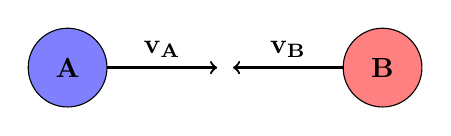
\begin{tikzpicture}

% Draw the first object (Object A)
\draw[<-, thick] (2.1, 0) -- (3.5, 0) node[midway, above] {$\mathbf{v_B}$};
\draw[fill=blue!50] (0,0) circle (0.5);
\node at (0, 0) {\textbf{A}};

% Draw the second object (Object B)
\draw[->, thick] (0.5, 0) -- (1.9, 0) node[midway, above] {$\mathbf{v_A}$};
\draw[fill=red!50] (4,0) circle (0.5);
\node at (4, 0) {\textbf{B}};

\end{tikzpicture}

\vspace{1cm}

% After the collision (Elastic)
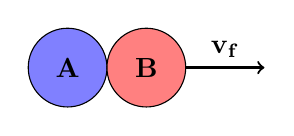
\begin{tikzpicture}
	\draw[fill=blue!50] (0,0) circle (0.5);
	\node at (0, 0) {\textbf{A}};
	\draw[fill=red!50] (1,0) circle (0.5);
	\node at (1, 0) {\textbf{B}};
	\draw[->, thick] (1.5, 0) -- (2.5, 0) node[midway, above] {$\mathbf{v_f}$};
\end{tikzpicture}

% Pendulum at Rest with Bullet Approaching
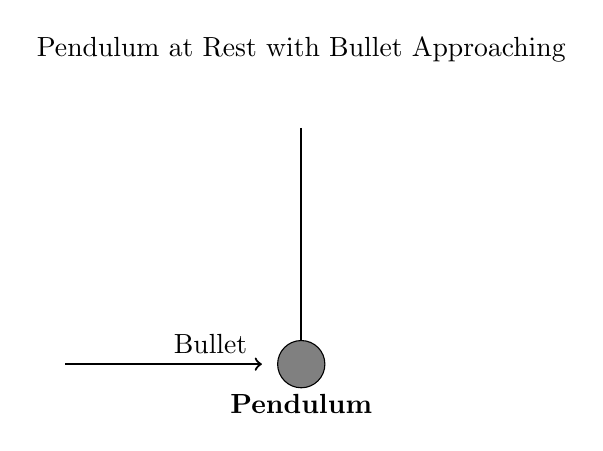
\begin{tikzpicture}
    % Pendulum
    \draw[thick] (0,0) -- (0,-3) ;
		\node at (0, -3.5) {\textbf{Pendulum}};
    \draw[fill=black!50] (0,-3) circle(0.3); % Pendulum bob

    % Bullet approaching
    \draw[thick, ->] (-3,-3) -- (-0.5,-3) node[midway, above right] {Bullet};

    % Label for the first image
    \node at (0, 1) {Pendulum at Rest with Bullet Approaching};
\end{tikzpicture}

\bigskip

% Pendulum Swinging Back with Bullet Lodged Inside
\begin{tikzpicture}
    % Pendulum
    \draw[thick] (0,0) -- (2.3,-3) 
    \draw[fill=black!50] (2.3,-3) circle(0.3); % Pendulum bob
	\node at (4, -2.5) {\textbf{Pendulum with bullet}};
    % Bullet lodged inside the pendulum
    \draw[thick, fill=gray] (2,-3) circle(0.1); % Bullet inside bob

    % Swinging motion (pendulum arc)
    \draw[thick, dotted] (0,-4) arc[start angle=-90, end angle=-45, radius=3];

    % Label for the second image
    \node at (0, 1) {Pendulum Swinging Back with Bullet Lodged Inside};
\end{tikzpicture}
\[
m_av_a + m_bv_b=\left( m_a+m_b \right) v_f
.\] 
\[
r=\frac{ \text{ Relative speed after collision } }{ \text{ Relative speed before collision } } = 0
.\] 
\[
\Delta KE= \frac{ m_am_b }{ 2\left( m_a+m_b \right)  }\left( v_a-v_b \right) ^2
.\] 
\newpage
\section{Read me}%
\label{sec:Read me}

Completely inelastic collisions occur when two objects collide like the picture below, and stick together, moving as one mass, leading to the bottom diagram. After the collision the momentum in the system will be the same as before the collision leading to the above equation on the left, but the kinetic energy will not be conserved. This goes on to state the difference between just inelastic and completely inelastic. During a regular inelastic collision, objects will move in the same direction but not completely as the same object. This often occurs with car crashes as their collisions will often lead to the energy loss ratio being between 0 and 1, non-inclusive, other than some very special cases that are hard to replicate in a non controlled environment. These special cases are completely inelastic when the ratio will equal 0, and completely elastic when the ratio will equal 1. It's important to note though that just because the ratio will equal 0, that doesn't mean that ALL kinetic energy will be lost, and instead will be the max amount that can be lost while still retaining the original momentum. 

\subsection{Next slide}%
\label{sub:Next slide}
For example, this is a completely inelastic collision where kinetic energy is not conserved. The picture on the left shows a ballistic pendulum used for testing bullet and gun velocities being approached by a bullet and the right shows the afteraffects of the bullet impacting the pendulum. This is an example of a completely inelastic collision because all of the kinetic energy from the bullet will be converted to heat, sound, and deformation of the bullet and pendulum. This leads to the bullet being lodged inside the pendulum and moving with the same vector as the pendulum. The below equation is the general equation for finding the delta in kinetic energy between the start and ending kinetic energy and it is at it's maximum because during completly inelastic collisions the most amount of kinetic energy will be lost while conserving the initial momentum of the system. 
\subsection{Next slide}%
\label{sub:Next slide}
As a recap, the 3 main things needed for a completely inelastic collision is the conservation of momentum, which occurs when the top equation is true, when kinetic energy loss is at it's maximum, which can be found using the middle equation, and when the objects stick together and move along the same vector after the collision.
\end{document}
